\section{SVM}
\subsection{Binary classification}
\begin{frame}{Binary classification}
	\begin{itemize}\setlength\itemsep{1em}
		\item[Goal:] To produce a classifier able to decide whether an object belongs to one or more classes.
		\item[Idea:] Supervised Learning: Given a dataset of already classified examples, the classifier \textit{learns} a function that solves classification problem.
	\end{itemize}
\end{frame}

\begin{frame}{Notation}
	\begin{itemize}\setlength\itemsep{1em}
		\item A vector $x \in \mathbb{R}^f$ represents an object using $f$ \textit{relevant} features.
		\item A vector $y \in \{-1 , +1\}^l$ indicates wether the example belong to each of the $l$ label classes.
	\end{itemize}
	The input of a classification problem is a dataset $D = \{X, Y\}$ where $X \in \mathbb{R}^{n\times f}$ is a set of examples and $Y \in \mathbb{R}^{n\times l}$ is a set of labels.
	
	While learning the target function, the dataset is divided in \textit{training set} and \textit{test set}.
\end{frame}

\subsection{SVM}
\begin{frame}{SVM}
	\begin{itemize}\setlength\itemsep{1em}
		\item For 1-class problems we have to compute the \textit{maximum-margin hyperplane} $w^Tx + b$ which best separates positive examples from negative examples.
	\end{itemize}
	Optimization problem is:
	\begin{columns}
		\begin{column}{0.5\textwidth}\centering
			$$arg min_w \frac{1}{2} ||w||^2$$
			$$y^{(i)} (w^T x^{(i)} + b) \geq 1 \ \forall i \in [1, n]$$
		\end{column}
		\begin{column}{0.5\textwidth}\centering
			\begin{figure}[htbp]
				\centering
				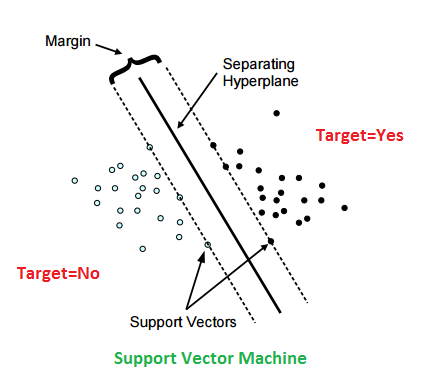
\includegraphics[scale = 0.40]{./images/optimal-hyperplane2.png}
				\caption{\textit{Solution of maximum-margin hyperplane}}
			\end{figure}
		\end{column}
	\end{columns}
	
	
	
\end{frame}

\begin{frame}{SVM with slacks}
	\begin{itemize}\setlength\itemsep{1em}
		\item The examples may not be linearly serparable and so the problem would not have any solutions because constraints are not satisfied. Then we introduce slack variables $\xi$
	\end{itemize}
	Optimization problem becames:
	\begin{columns}
		\begin{column}{0.5\textwidth}\centering
			$$arg min_{w, \xi} \frac{1}{2} ||w||^2 + C \sum_{i = 1}{n}\xi^{(i)}$$
			$$y^{(i)} (w^T x^{(i)} + b) \geq 1 - \xi^{(i)} \ \forall i \in [1, n]$$
			$$\xi^{(i)} \geq 0 \ \forall i \in [1, n]$$
		\end{column}
		\begin{column}{0.5\textwidth}\centering
			\begin{figure}[htbp]
				\centering
				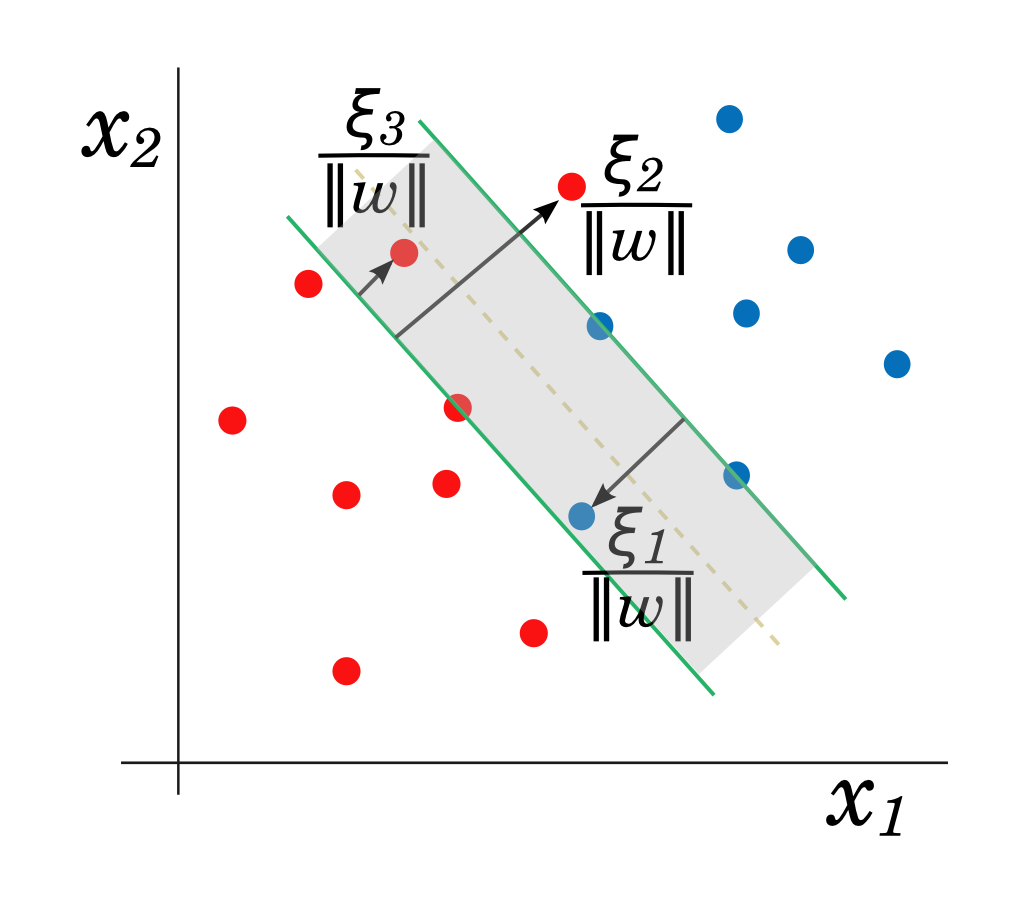
\includegraphics[scale = 0.15]{./images/slack2.png}
				\caption{\textit{Solution with slacks}}
			\end{figure}
		\end{column}
	\end{columns}
	
\end{frame}